\chapter{Benchmarks and implementation details}
\section{Implementation details}
\subsection{KOALA NetworKit}
All of the algorithms described in this paper were implemented 
using \textsc{C++20} for an open-source KOALA NetworKit \cite{turowski_koala_networkit} library.

KOALA NetworKit joins two open-source libraries: KOALA and 
NetworKit library. At first we can get familiar with them by following 
README file from KOALA NetworKit repository \cite{turowski_koala_networkit}.

\begin{itemize}
    \item NetworKit \cite{staudt2016networkit} is an open-source general purpose networking analysis
        and graph mining library written in \textsc{C++}. Graphs are 
        represented in a compact form, while preserving the efficiency 
        of changes to their structure such as node and edge additions 
        and deletions. The library contains algorithms mostly for 
        the structural analysis of massive complex real-world networks,
        but lacks some of the most important general graph algorithms like 
        graph coloring.
    \item In places where NetworKit library is lacking, KOALA \cite{dobrowolski2008koala} library excells.
        It is an open-source library of C++ templates, developed at Gdansk 
        University of Technology Department of Algorithms and System Modeling.
        Its main part consists of an implementation of a broad set of 
        procedures in algorithmic graph theory and network problems in discrete 
        optimization. The library contains algorithms for problems like: graph coloring, 
        graph search, flow problems, graph recognition for graph families and many more.
\end{itemize}

Because KOALA NetworKit is a fork of KOALA library built on structures provided 
by NetworKit, it combines the best of two worlds by providing a simple, fast 
and powerful unified interface for a broad class of algorithms.

The contribution of this work to the KOALA NetworKit library are 
mainly in the following files:
\begin{itemize}
    \item \texttt{cpp/techniques/separator/LiptonTarjanPlanarSeparator.cpp}
        and \texttt{cpp/techniques/separator/LiptonTarjanFundamentalCycle.cpp}
        provide an efficient $O(n)$ implementation of Lipton-Tarjan planar 
        separator algorithm discussed in \Cref{sec:planar-sep}
    \item \texttt{cpp/techniques/separator/MISP.cpp} provides the implementation 
        of \Cref{alg:epsilon-planar-separator} and \Cref{alg:MISP} for further use
        in other algorithms
    \item \texttt{cpp/vertex\_cover/PlanarVertexCover.cpp} provides the implementation 
        of approximation algorithm for Vertex Cover Problem (\Cref{alg:prep} and \Cref{alg:bipartite})
    \item \texttt{cpp/matching/PlanarMaximumMatching.cpp} provides the implementation of
        approximation algorithm for Maximum Matching Problem (\Cref{alg:matching})
\end{itemize}
\subsection{Lipton-Tarjan planar separator algorithm}
Implementation of this algorithm uses an embedding algorithm provided by KOALA NetworKit
library that is based on Boyer-Myrvold $O(n)$ embedding algorithm from Boost \cite{boost} library.
The critical section of this algorithm which is \Cref{alg:fundamental_cycle} is based
on two \texttt{EdgeScanner} structures that allows for scanning edges in two directions 
of the cycle one at a time, which is the cornerstone of $O(n)$ implementation. Moreover, 
in order to update the cycle structure in $O(1)$ time at the of each iteration, it is 
implemented as a double linked list to ensure quick splicing and merging.

\subsection{\textsc{MISP} algorithm}
This algorithm is implemented as a generic class \texttt{MISP<T>}, so that it supports both 
vertex and edge sets for Vertex Cover and Maximum Matching Problems respectfully. In order to 
achieve the theoretical $O(n\log n)$ time complexity, the graphs are compacted and remapped 
during each iteration of the algorithm using methods from KOALA NetworKit library.

\subsection{Vertex Cover algorithm}
This algorithm faithfully follows the pseudocode provided in listings for \Cref{alg:prep} and
\Cref{alg:bipartite}. It is worth noting, that to minimize the effect of graph compacting and 
mapping, it has been decided, to abandon it for this algorithm, which changes the time complexity
of \Cref{alg:prep} to $O(n \log n)$ instead of $O(n)$ guaranteed by theoretical analysis. However, 
it is not a major issue, as \textsc{MISP} already has $O(n \log n)$ time complexity which is 
a bottleneck for the algorithm.

\subsection{Maximum Matching algorithm}
Implementation of this algorithm follows the pseudocode provided in listing for \Cref{alg:matching}.
However, to avoid problems with stack memory during recursive calls of the algorithm, it has been decided
to abandon its recursive structure in favor of splitting the algorithm into two parts. The first one 
is reduction phase, where we keep track of vertices that take part in each reduction onto a separate stack
vector. After reduction phase is finished, the exact solution is found using \textsc{MISP} algorithm. The final
phase of the algorithm is backtracking and retrieving the matching using the stack.

\section{Benchmark structure and results}
The benchmarks have been run for two approximation algorithms: Vertex Cover algorithm and Maximum Matching algorithm, 
as well as a separate benchmark for Lipton-Tarjan planar separator algorithm itself. The benchmarks consisted of
six planar graph families:
\begin{itemize}
    \item cycle graphs - they represent cycles of length $n$
    \item grid graphs - square grids, with side lengths $\left \lfloor{\sqrt{n}}\right \rfloor$
    \item trigrid graphs - square grids, with side lengths $\left \lfloor{\sqrt{n}}\right \rfloor$ 
        such that every internal face is a triangle
    \item hexagonal grid graphs - grids, with side lengths $\left \lfloor{\sqrt{n}}\right \rfloor$
        such that every face is a hexagon (a cycle of length $6$)
    \item tree graphs - random trees with $n$ vertices, where each vertex is randomly (with uniform distribution) attached 
        to some other vertex already present in a graph
    \item apollonian graphs - a maximal planar graph of $n$ vertices that is created by following a simple algorithm

\begin{algorithm}[H]
\caption{\textsc{APOLLONIAN} procedure}
\label{alg:apollonian}
\begin{algorithmic}[1]
\Require $n \colon \text{number of vertices}$
\Ensure $G \colon \text{graph}$
\State $G \gets \text{triangle}$
\While{$|V(G)| < n$}
\State Select a face $F = (u,v,w)$ uniformly at random
\State Add a new vertex $x$ to $G$
\State Add edges $(x,u)$, $(x,v)$, and $(x,w)$ to $G$
\EndWhile
\State \Return $G$
\end{algorithmic}
\end{algorithm}

\end{itemize}

\begin{figure}[H]
\centering
    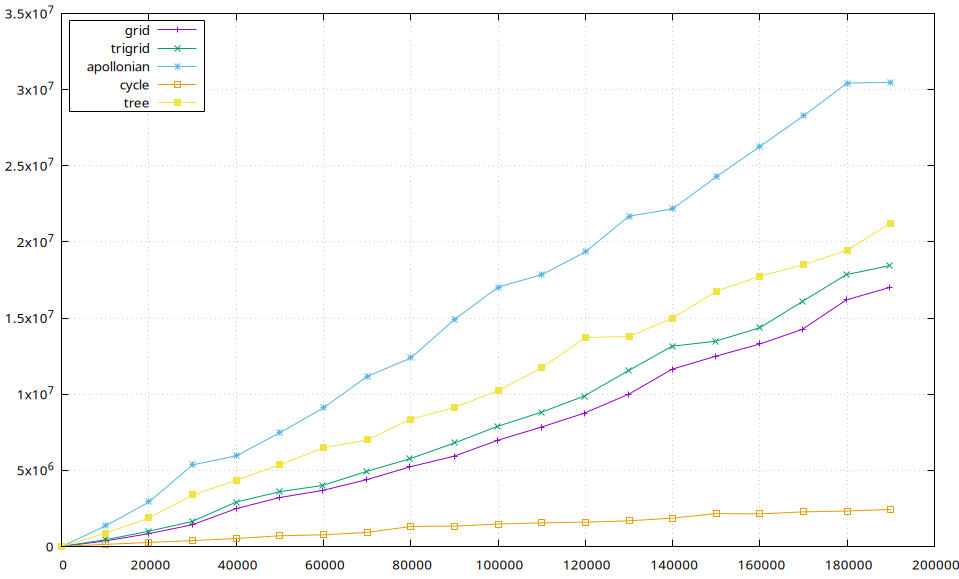
\includegraphics[width=0.85\textwidth]{plots/benchmark_combined.png}
    \caption{Lipton-Tarjan separator algorithm running time comparison}
    \label{fig:lt_sum}
\end{figure}

\begin{figure}[H]
    \centering
    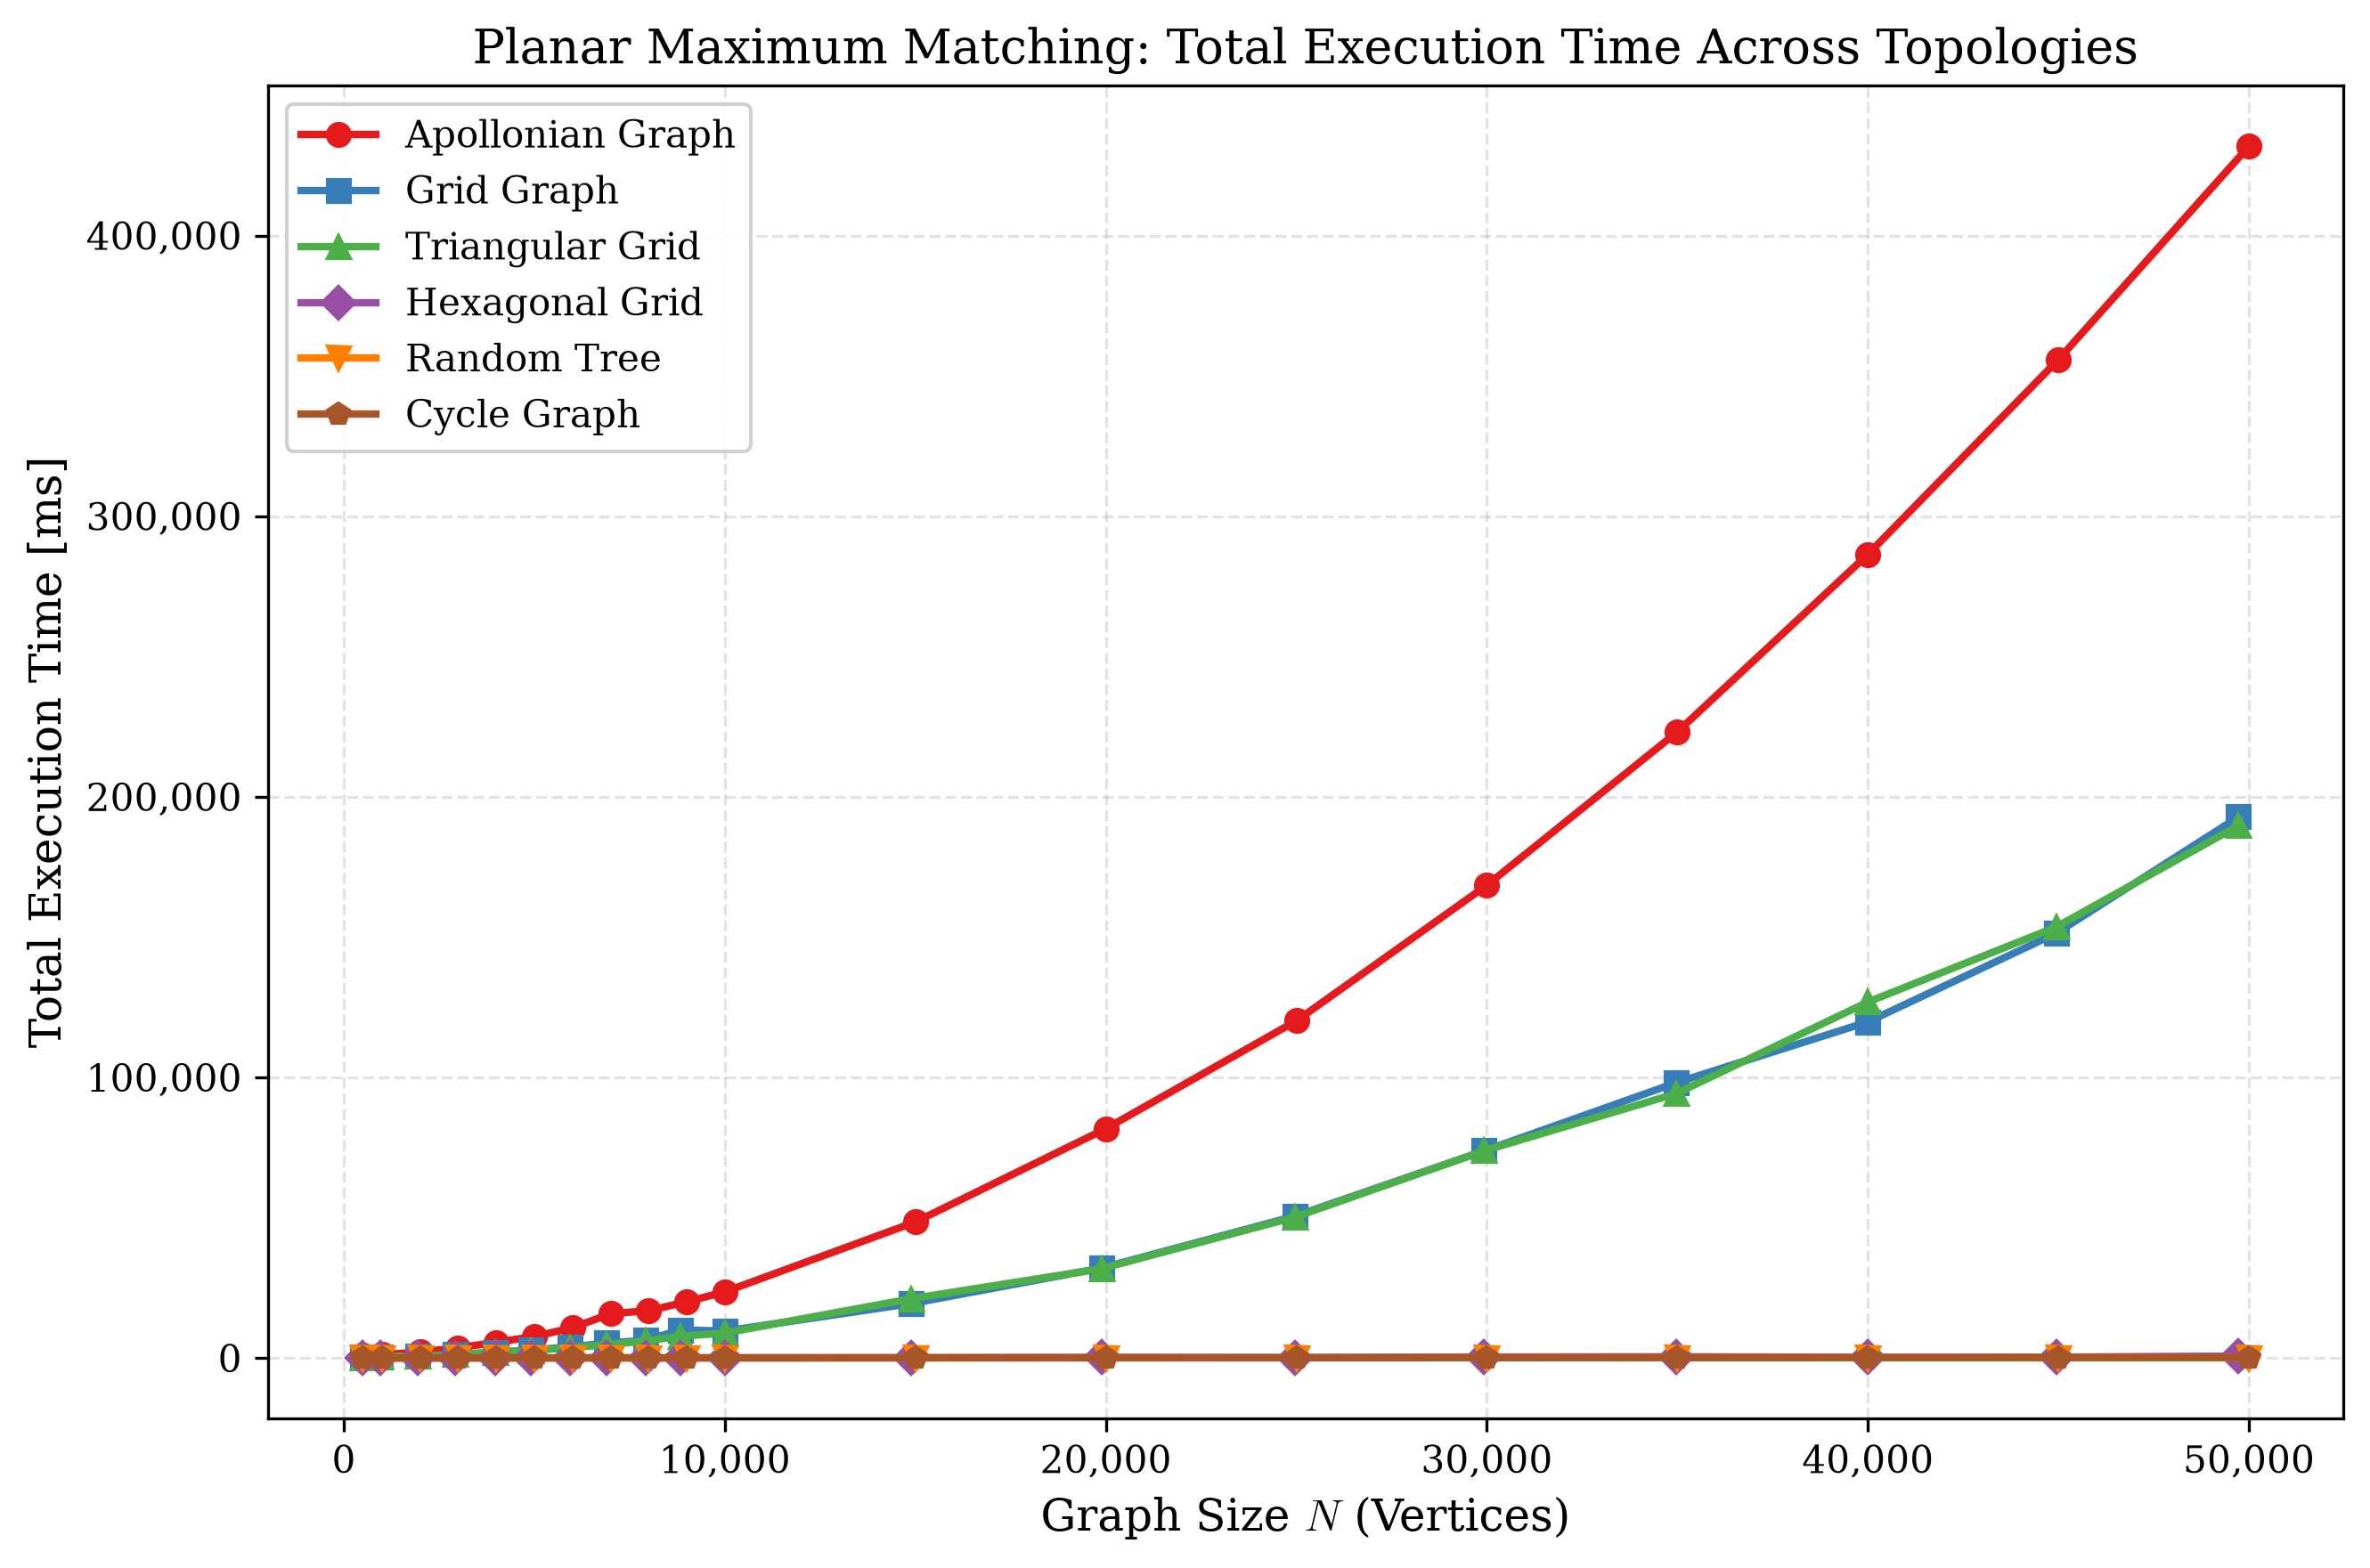
\includegraphics[width=0.85\textwidth]{plots/matching/cross_topology_comparison/cross_01_total_time_linear.png}
    \caption{Matching algorithm total running time comparison}
    \label{fig:match_total}
\end{figure}

\begin{figure}[H]
    \centering
    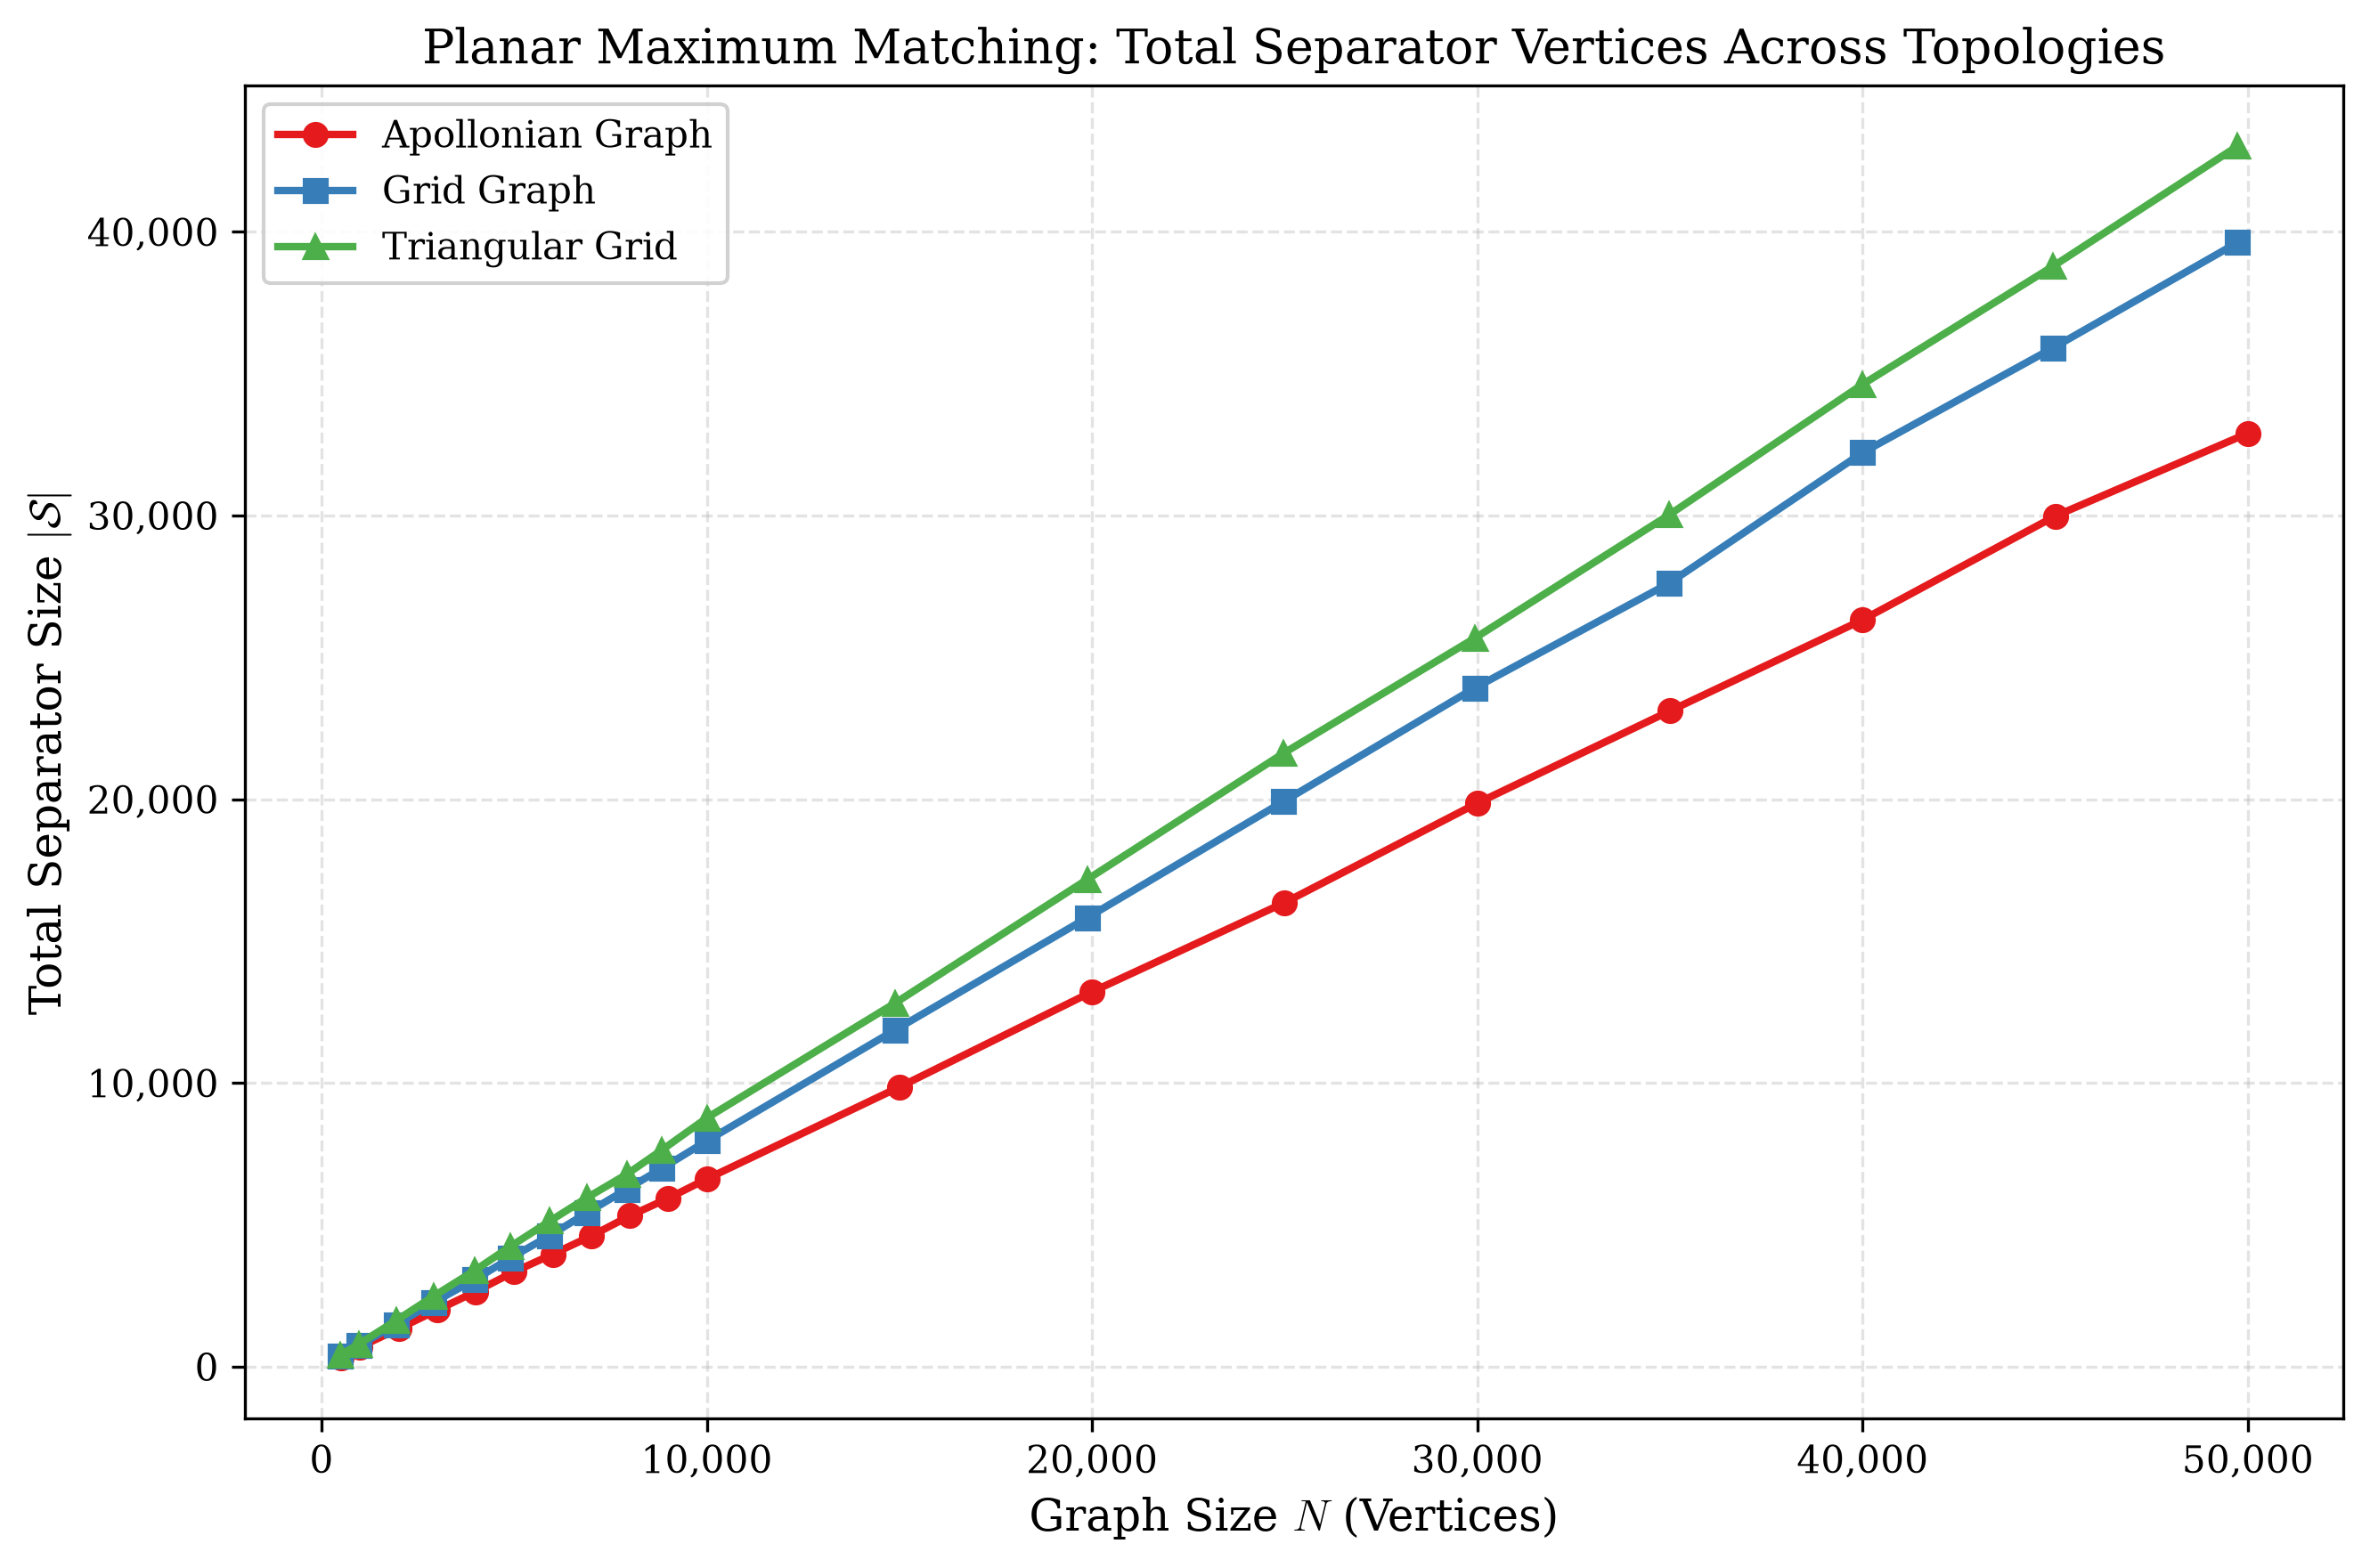
\includegraphics[width=0.85\textwidth]{plots/matching/cross_topology_comparison/cross_04_separator_nodes.png}
    \caption{Matching algorithm separator size comparison}
    \label{fig:match_sep_size}
\end{figure}

\begin{figure}[H]
    \centering
    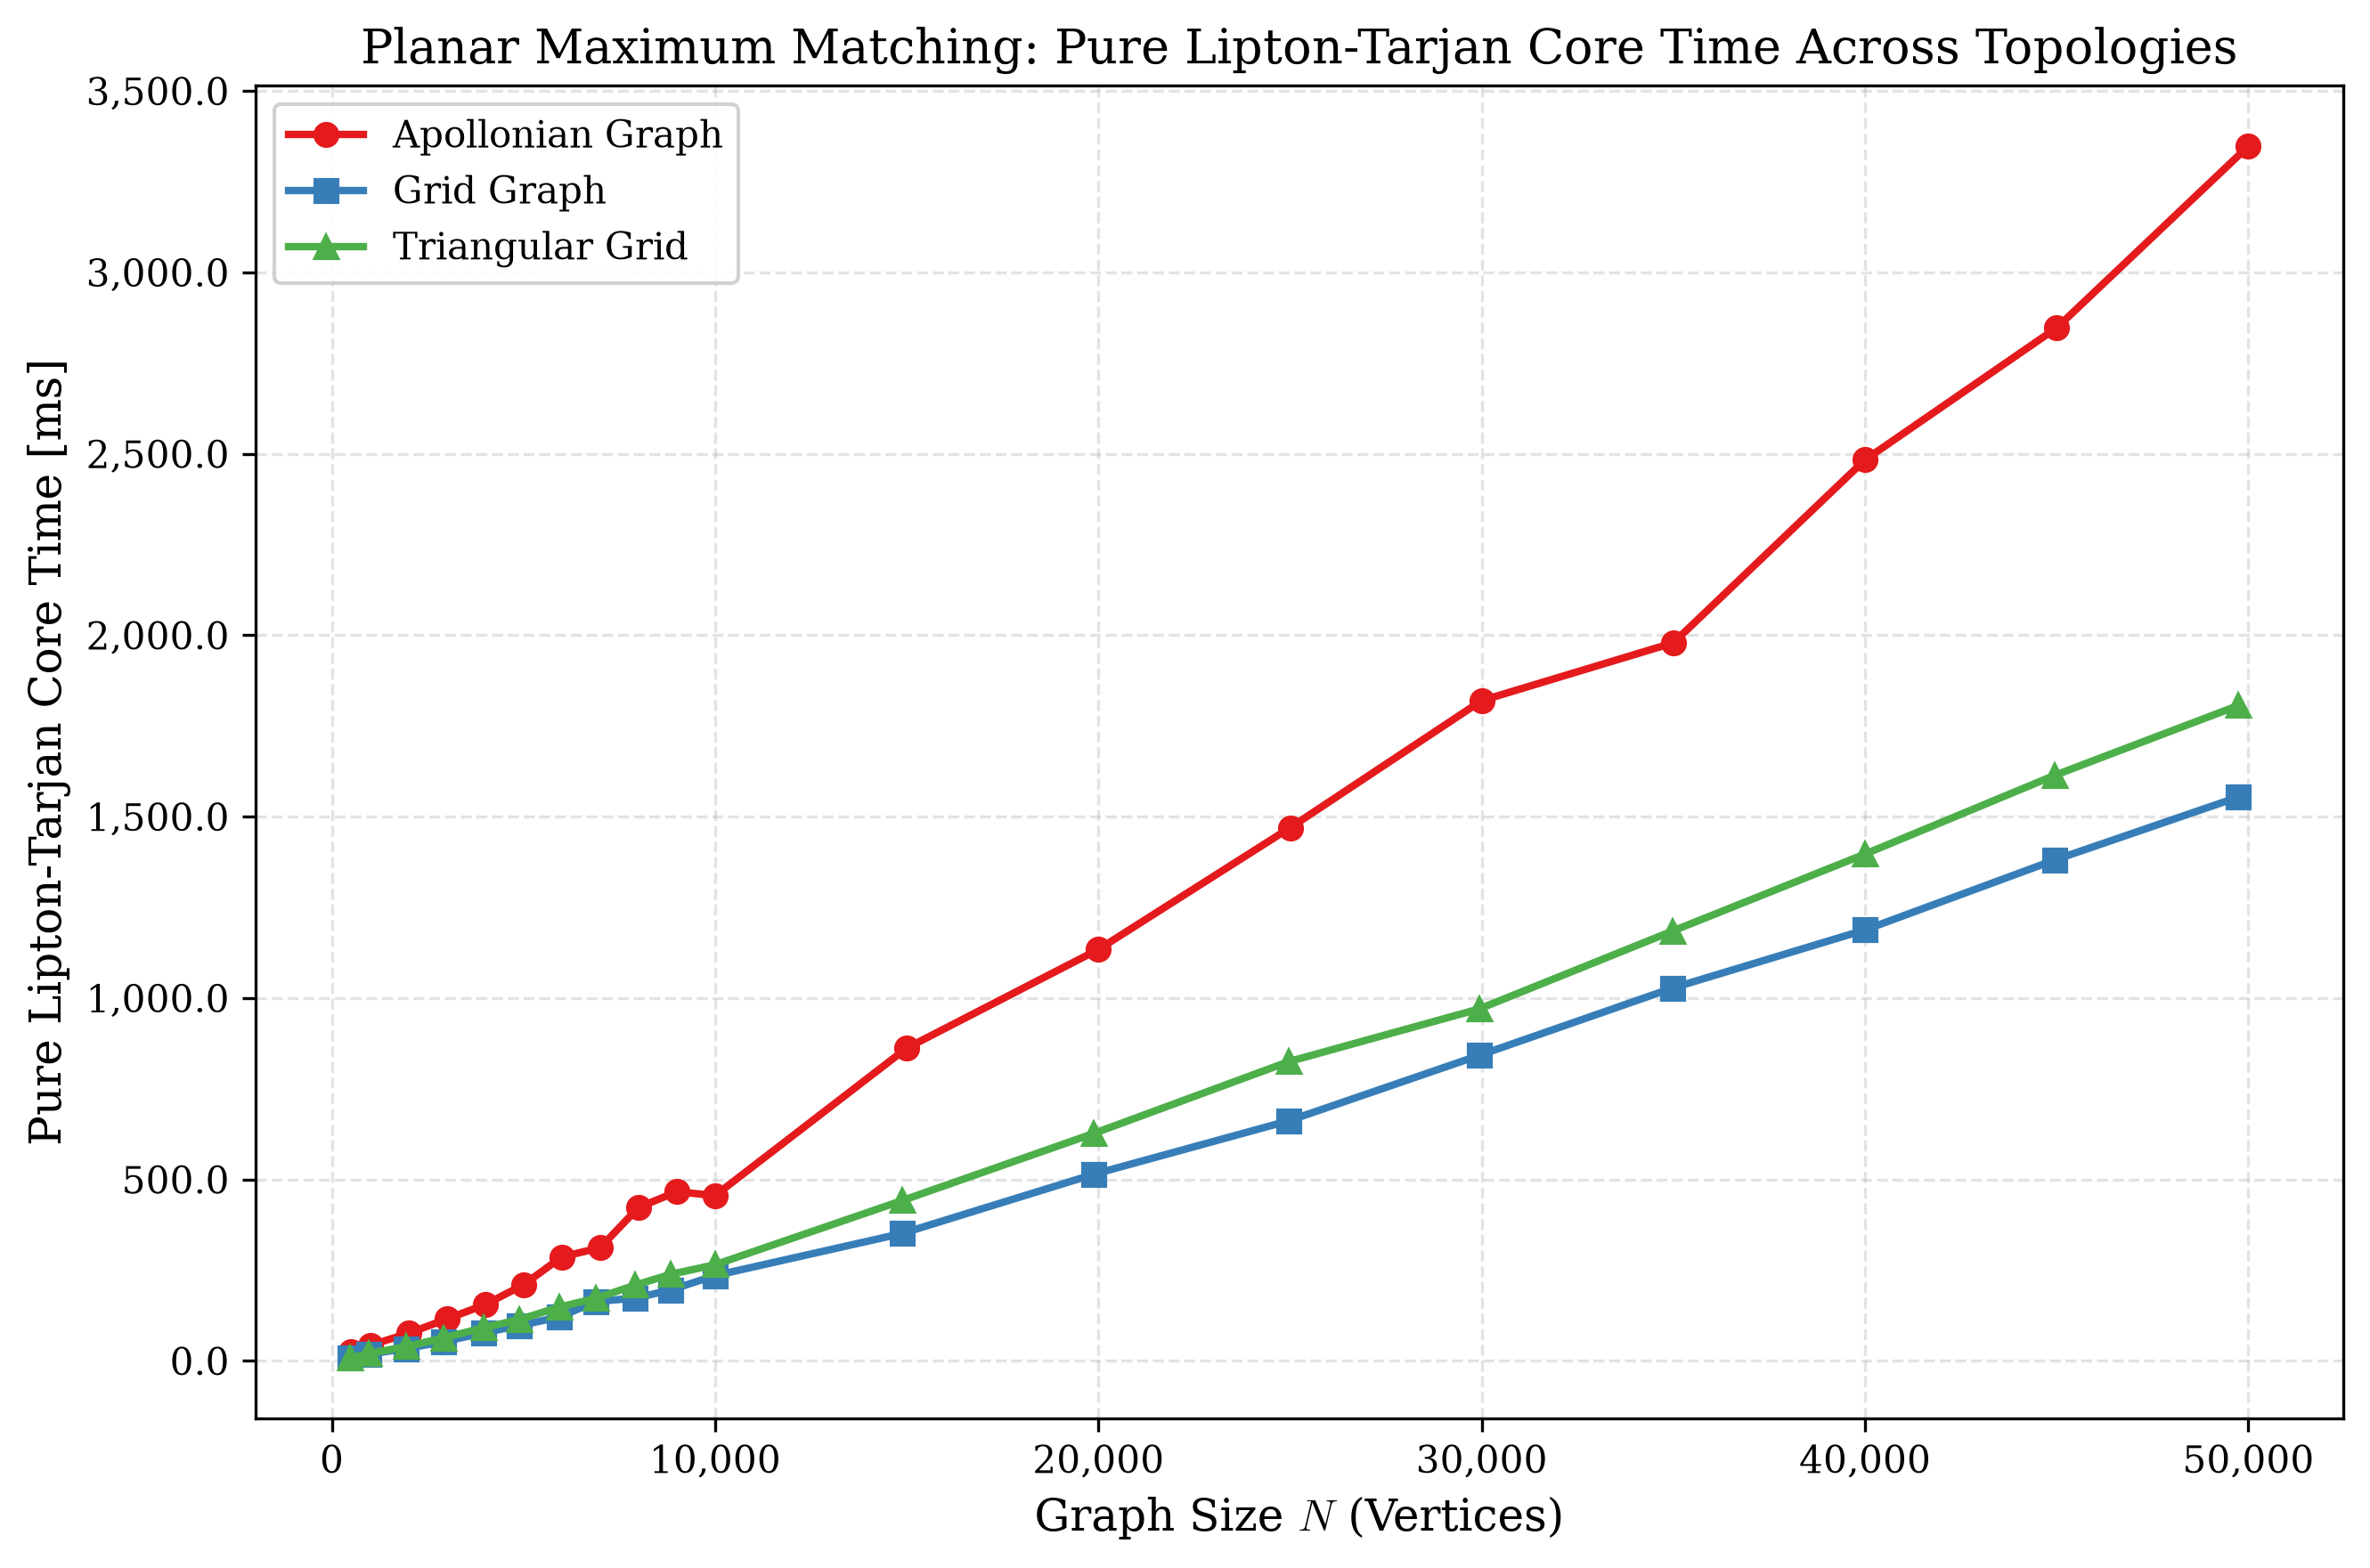
\includegraphics[width=0.85\textwidth]{plots/matching/cross_topology_comparison/cross_03_pure_lt_time_linear.png}
    \caption{Matching algorithm, separator algorithm running time comparison}
    \label{fig:match_sep_time}
\end{figure}
\begin{figure}[H]
    \centering
    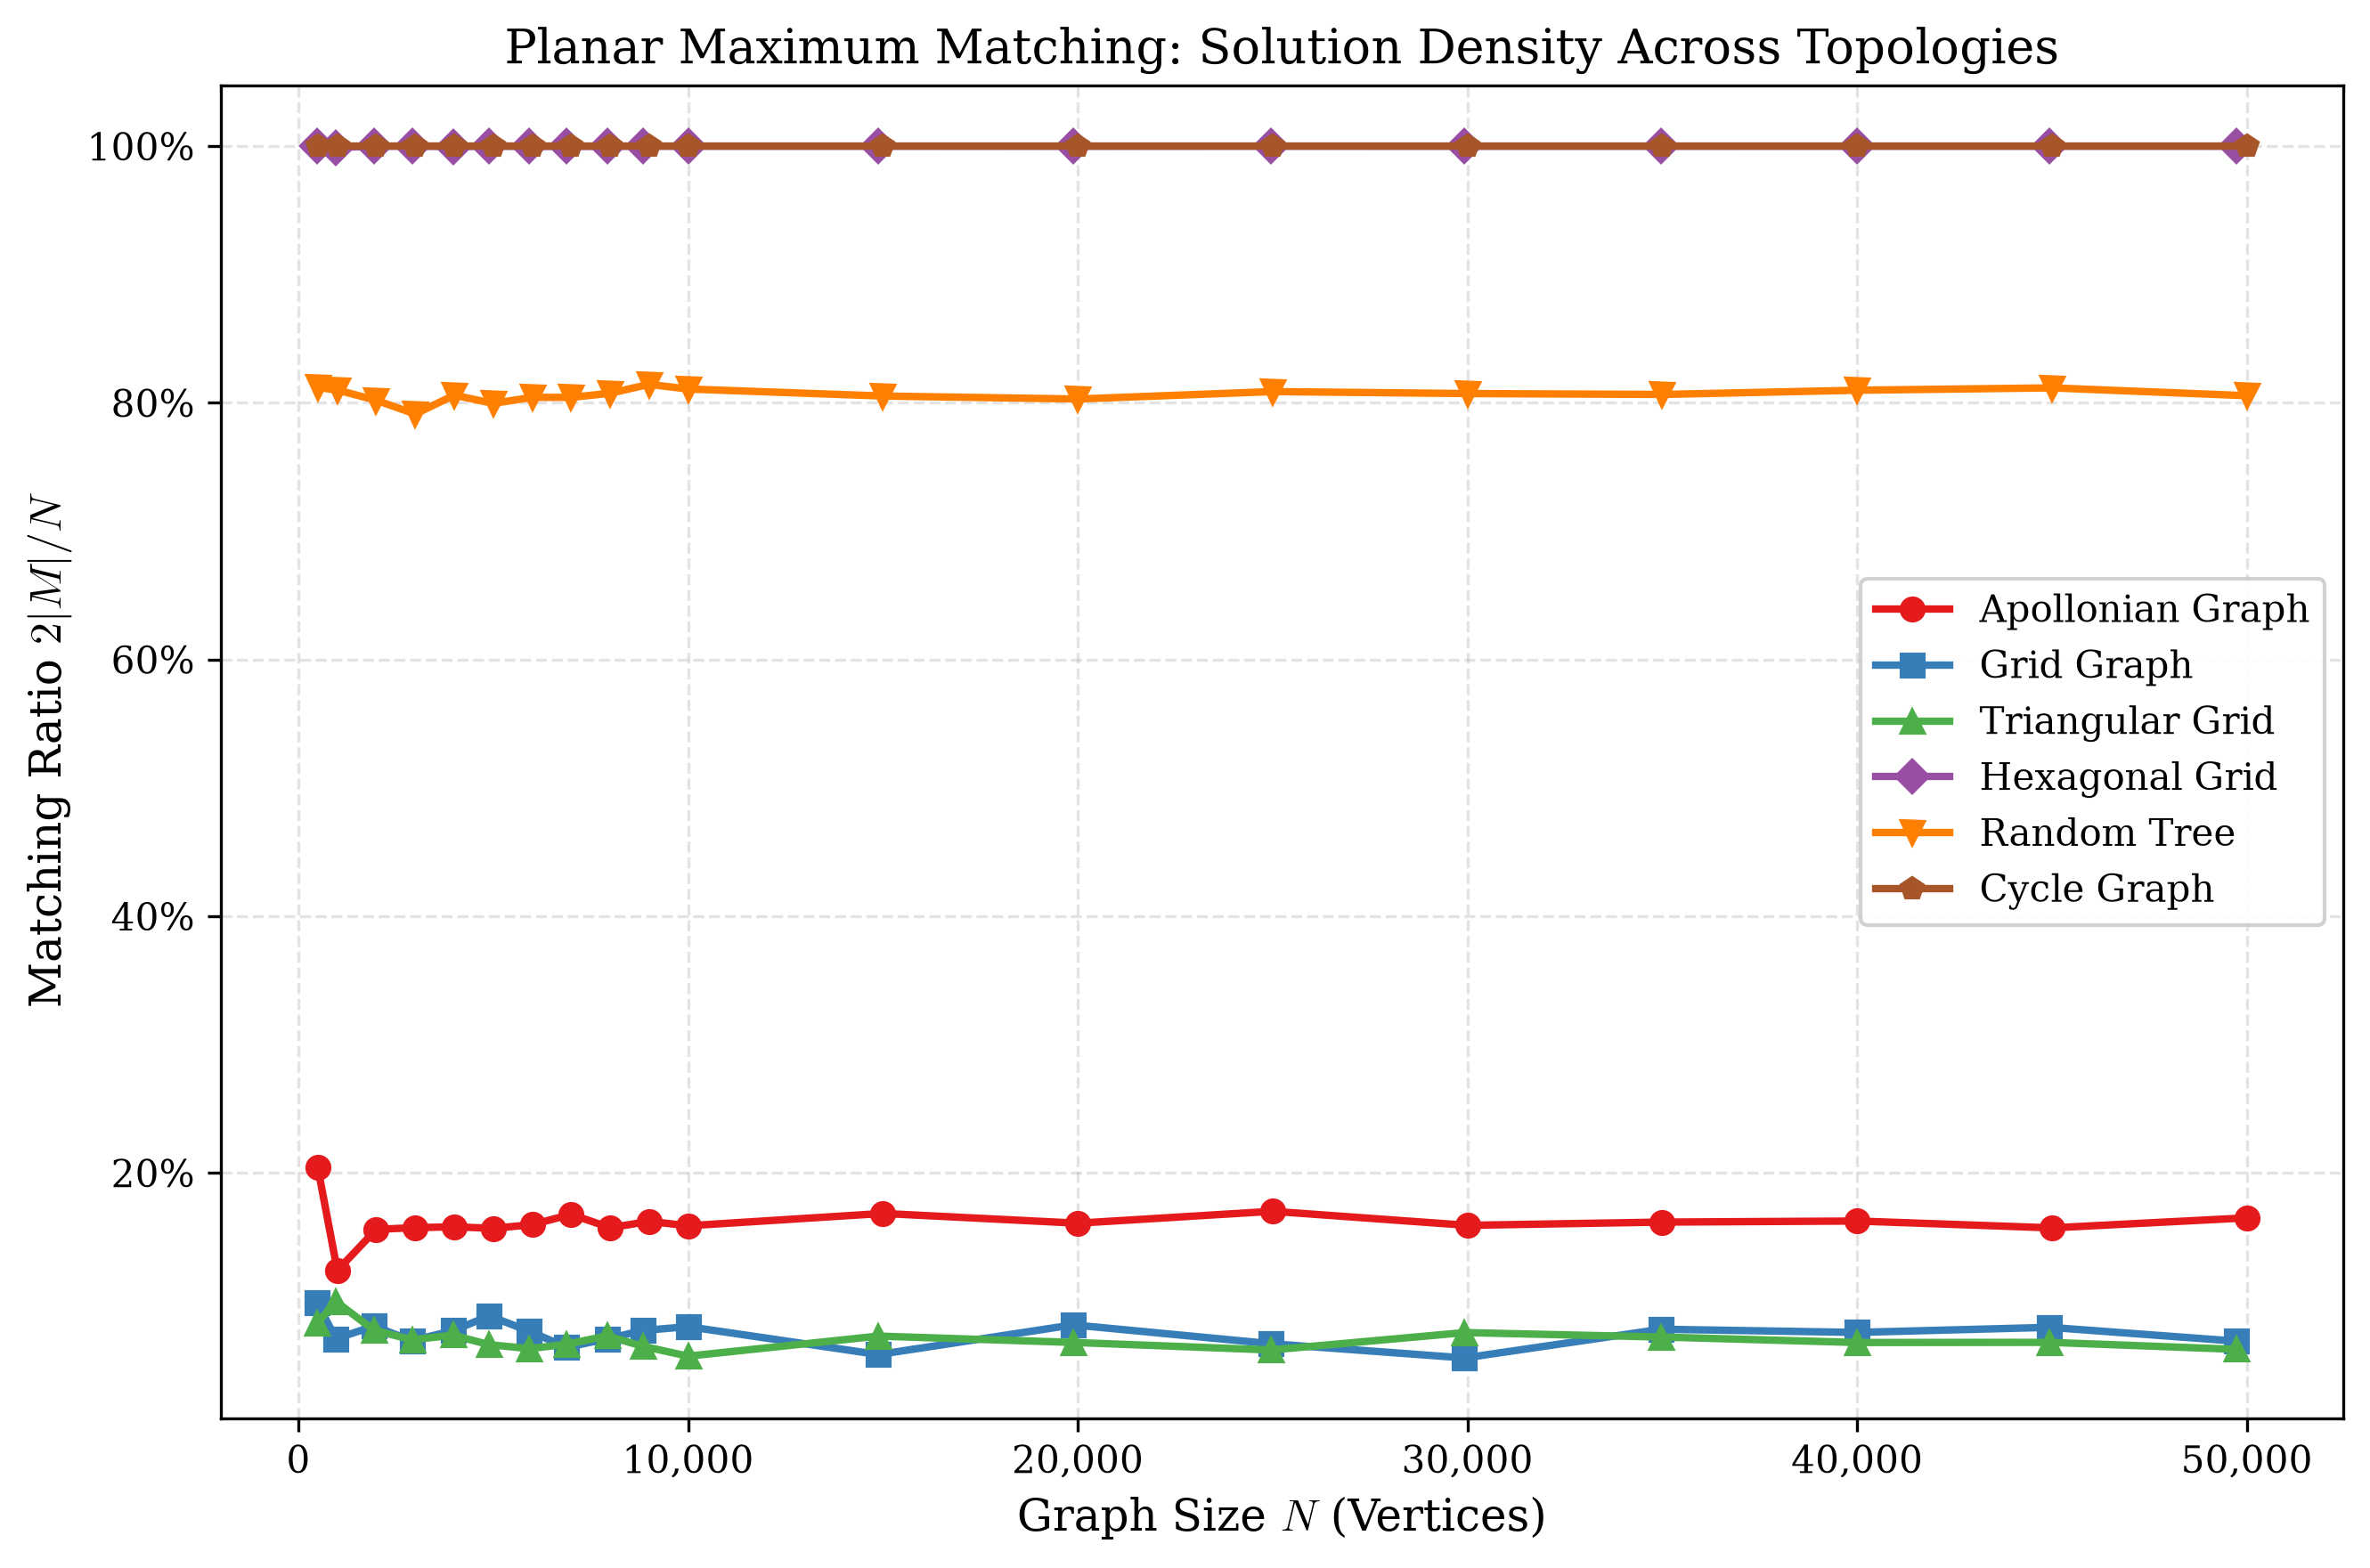
\includegraphics[width=0.85\textwidth]{plots/matching/cross_topology_comparison/cross_05_solution_ratio.png}
    \caption{Matching algorithm percentage of node covered}
    \label{fig:match_cover}
\end{figure}

\begin{figure}[H]
    \centering
    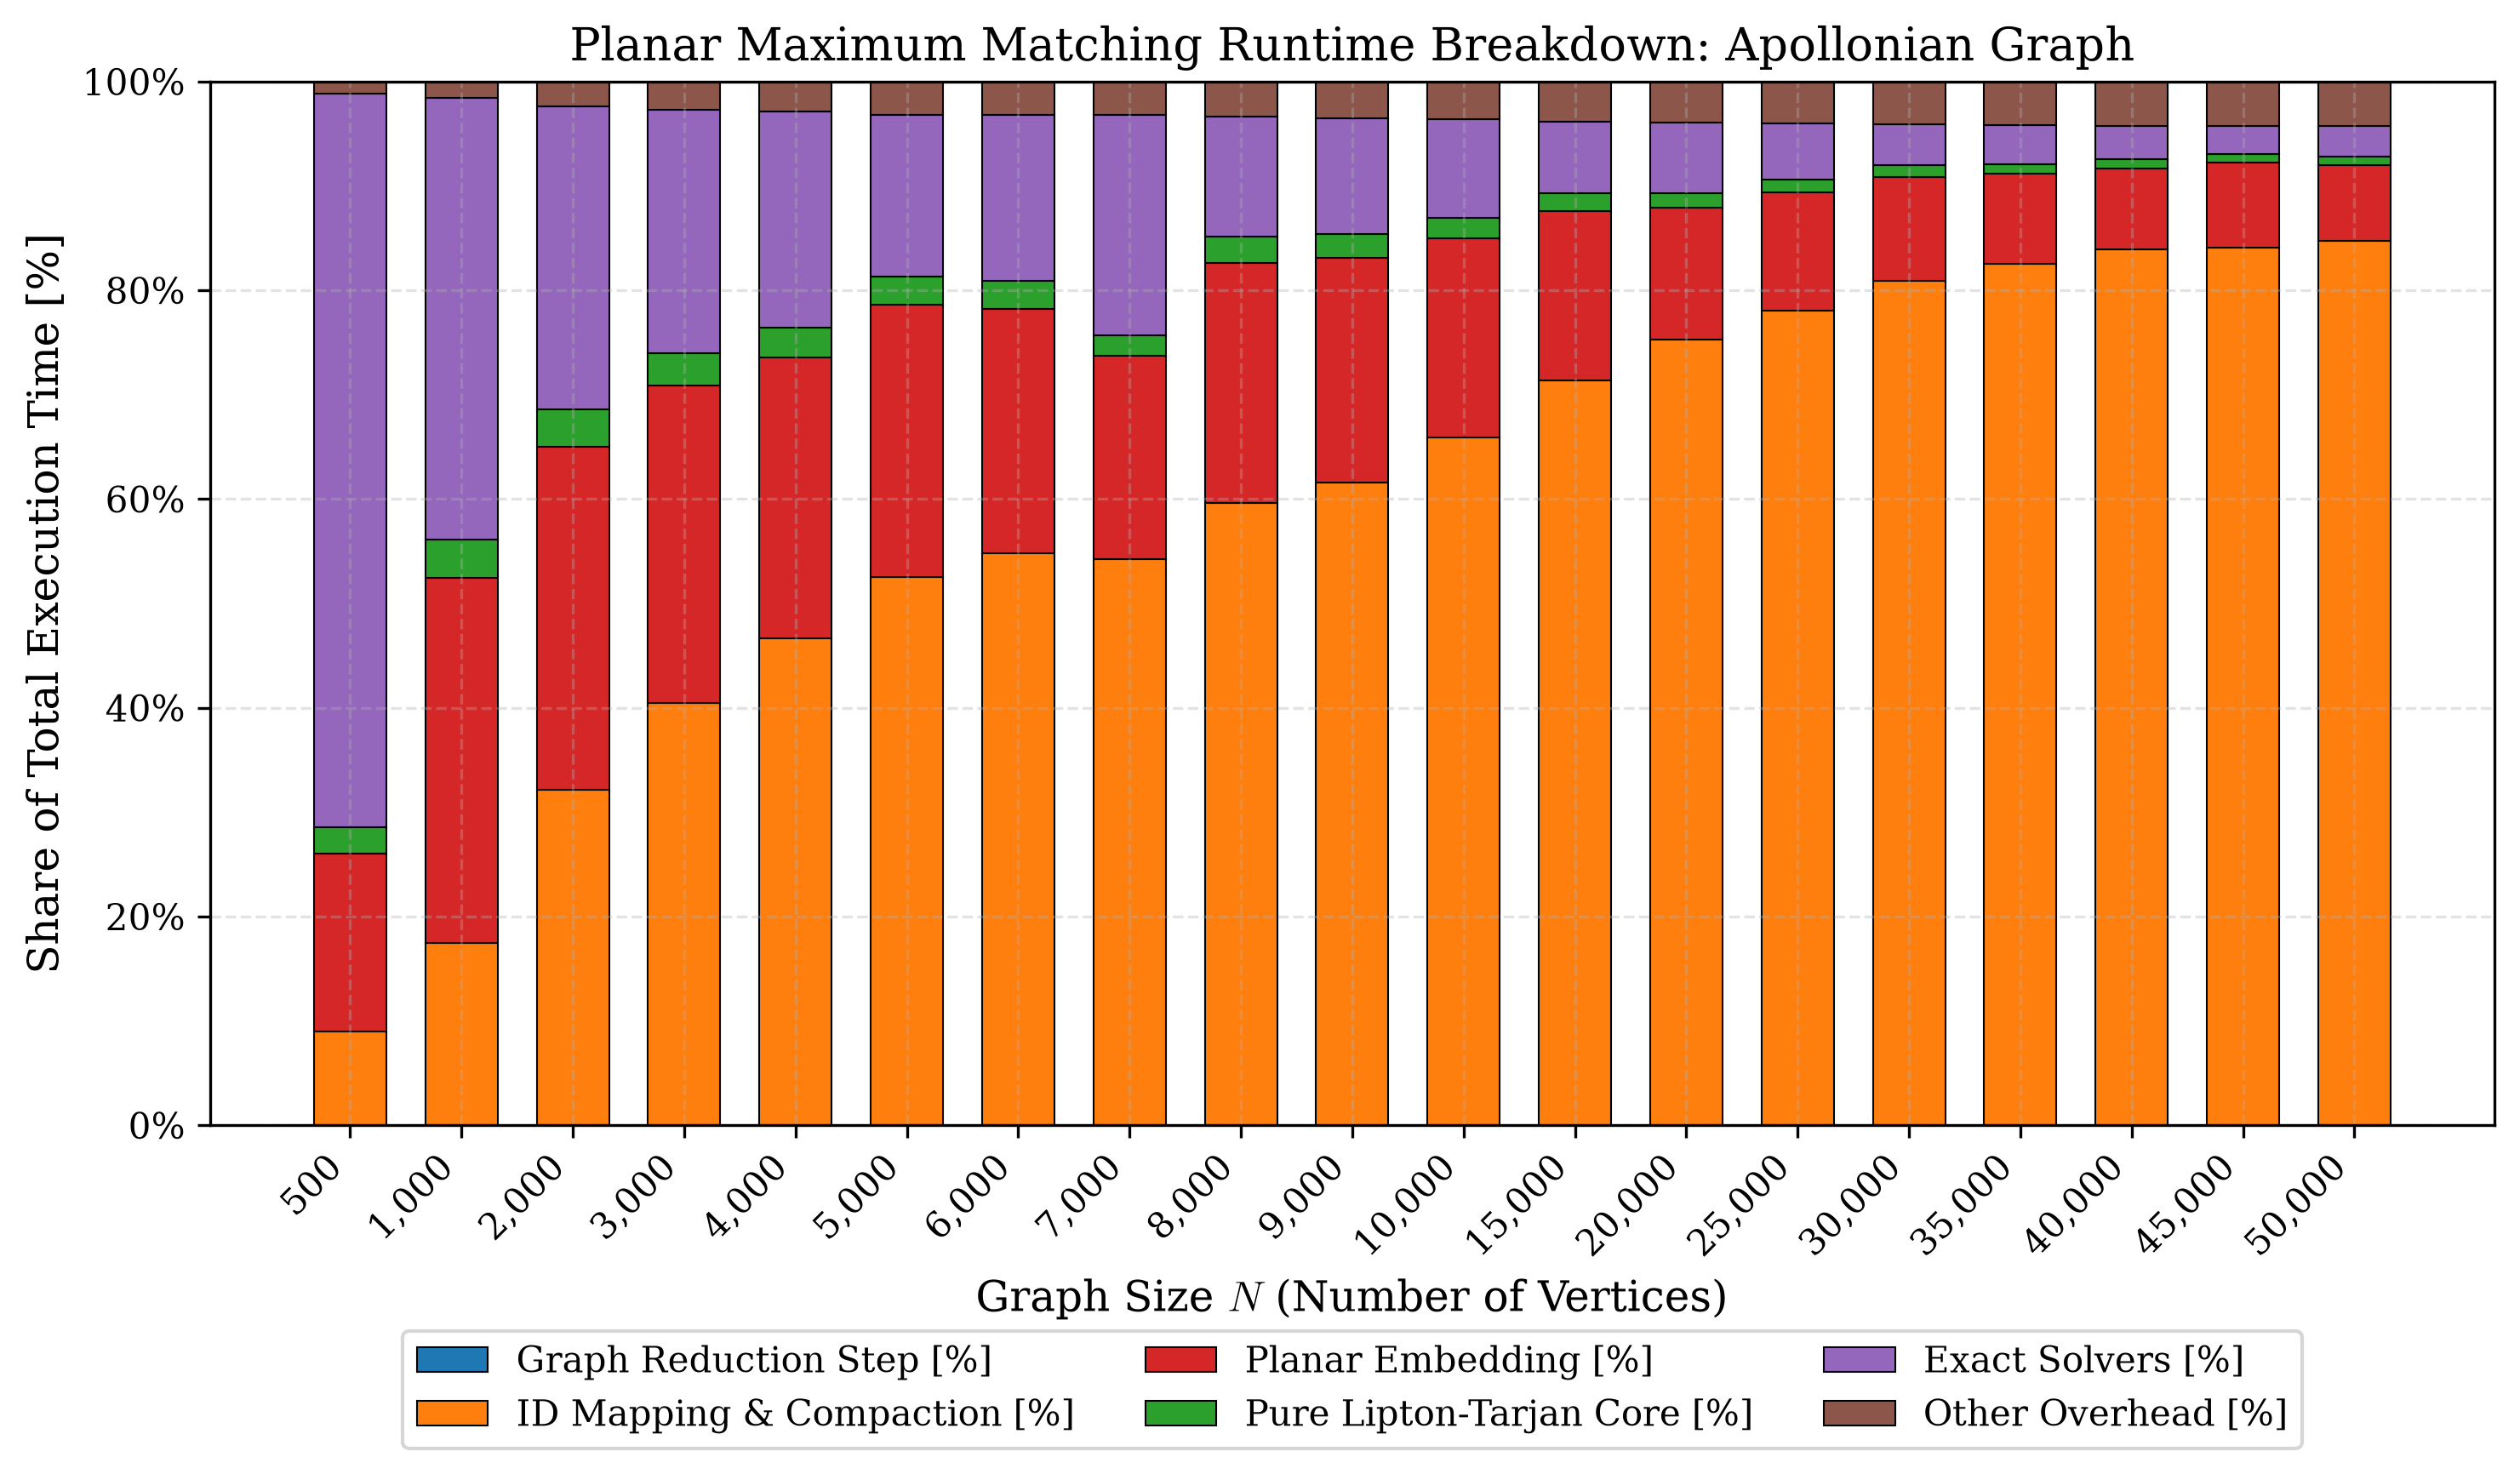
\includegraphics[width=0.85\textwidth]{plots/matching/apollonian_graph/01_percentage_breakdown.png}
    \caption{Matching algorithm percentage breakdown of different phases for apollonian graphs}
    \label{fig:match_perc}
\end{figure}

\begin{figure}[H]
    \centering
    
\includegraphics[width=0.85\textwidth]{plots/vertex_cover/cross_topology_comparison/cross_01_total_time_linear.png}
    \caption{Vertex Cover algorithm total running time comparison}
    \label{fig:vc_total}
\end{figure}

\begin{figure}[H]
    \centering
    
\includegraphics[width=0.85\textwidth]{plots/vertex_cover/cross_topology_comparison/cross_04_separator_nodes.png}
    \caption{Vertex Cover algorithm separator size comparison}
    \label{fig:vc_sep_size}
\end{figure}

\begin{figure}[H]
    \centering
    
\includegraphics[width=0.85\textwidth]{plots/vertex_cover/cross_topology_comparison/cross_03_pure_lt_time_linear.png}
    \caption{Vertex Cover algorithm, separator algorithm running time comparison}
    \label{fig:vc_sep_time}
\end{figure}

\begin{figure}[H]
    \centering
    
\includegraphics[width=0.85\textwidth]{plots/vertex_cover/cross_topology_comparison/cross_05_solution_ratio.png}
    \caption{Vertex Cover algorithm percentage of node covered}
    \label{fig:vc_cover}
\end{figure}

\begin{figure}[H]
    \centering
    
\includegraphics[width=0.85\textwidth]{plots/vertex_cover/apollonian_graph/01_percentage_breakdown.png}
    \caption{Vertex Cover algorithm percentage breakdown of different phases for apollonian graphs}
    \label{fig:vc_perc}
\end{figure}

From \Cref{fig:lt_sum} we can see that the total running time of isolated Lipton Tarjan planar separator algorithm
is linear, that aligns perfectly with what is expected from theoretical perspective. Moreover, we can see
that the size of a separator rises in linear manner (see \Cref{fig:match_sep_size} and \Cref{fig:vc_sep_size}).
If we recall \Cref{alg:epsilon-planar-separator} it guarantees 
a separator of size $O(n/ \epsilon)$, and in the case of our algorithms $\epsilon = \frac{\log\log n}{n}$ and because 
function $f(n) = \log\log n$ grows very slowly, for our small input we have linear progression. The next interesting thing
is how much time mapping and planar embedding takes when the size of input grows. We can see exactly that in \Cref{fig:match_perc} and 
\Cref{fig:vc_perc}. This brings a huge overhead on the total running time of the algorithm which can be seen in \Cref{fig:vc_total} and \Cref{fig:match_total}.
And for that the total running time of 
Lipton-Tarjan separator algorithms across all recursive calls has been measured, providing us with the real running time of the algorithm,
which can be seen in \Cref{fig:match_sep_time} and \Cref{fig:vc_sep_time}.

At last, we can look at \Cref{fig:match_cover} and \Cref{fig:vc_cover} which highlights how well does the approximation algorithm cover vertices and edges 
in respectful algorithms. Those plots highlight how difficult it is to measure theoretical approximation algorithms. As the approximation error of both algorithms 
is $O(\frac{1}{\sqrt{\log\log n}})$, for small sizes, that function is almost constant. Moreover as it had been mentioned in Section 3.1, by construction of 
\textsc{MISP} algorithm we lose all of the edges incident to vertices of a separator. And because the size of a separator increases linearly, for small graphs
many potential matching edges are lost. A better approach for an approximation matching algorithm based on a planar separator can be found in \cite{liptonApplicationsPlanarSeparator1977}.
